\section{Introduction}
\label{sec:introduction}

% Outline:
%  - Low-mass inspirals are the most promising source of gravitational radiation for advanced \textsc{ligo}
% - Motivation for high throughput
%   - Point out challenges of advanced detectors: more templates, longer templates
% - Motivation for low latency
%   - Observational applications of near-real-time detection
%   - Mention S6 and VSR2, online running, EM followup
% - Layout of paper: description of method, procedure followed 

\editorial{Would the introduction be more effective without this paragraph?, should we find whitepapers?}

The coalescence of compact binary systems consisting of neutron stars (NS)
and/or black holes (BH) is the most promising source of gravitational radiation
for Advanced \LIGO, Virgo, \GEO\ and \LCGT~\cite{ALIGOWeb, AVirgoWeb, GEOWeb,
LCGTWeb}.  Tens of binary coalescence events are expected to be observed in the
advanced detector era later this decade~\cite{Abadie:2010p10836}.

As a compact binary system loses energy to gravitational waves, its orbital
separation decreases. This causes a run-away inspiral with the
gravitational-wave amplitude and frequency increasing until the system
eventually merges near the innermost stable circular orbit (\ISCO).  If a
neutron star is involved it may become tidally disrupted near the merger.  This
disrupted matter can fuel a bright electromagnetic counterpart in the system's
final moments as a binary~\cite{shibata:2007}.

Prompt electromagnetic emission can arise as shells of relativistically
out-flowing matter collide in the inner shock. Such an inner shock from a
compact binary coalescence is believed to be a mechanism for short gamma-ray
bursts (short GRBs)~\cite{Lee:2005, nakar07}. The same inner shocks, or
potentially reverse shocks, can produce a bright accompanying optical flash~\cite{Sari99}. Prompt emission is a probe into the extreme
initial conditions of the outflow, in contrast with afterglows, which are
relatively insensitive to initial conditions. Optical flashes
have only been observed for a handful of long
GRBs~\cite{1999Natur.398..400A,2003Natur.422..284F,2006A&A...454L.119J,0004-637X-660-1-489,2008Natur.455..183R,2011A&A...528A..15G}
by telescopes with extremely rapid response or, in the case of GRB 080319B, by
pure serendipity, where several telescopes were observing a previous GRB in the
same field~\cite{2008Natur.455..183R}. Short GRBs, on the other hand, typically
fade too quickly to observe anything before the initial burst of gamma rays and hard
x-rays. Rapid gravitational-wave transient alerts could enable the observation
of optical flashes from short GRBs. An optical counterpart would vastly boost
confidence in the gravitational-wave detection and provide the tight sky
localization necessary to allow determination of the source's host galaxy,
which leads to a redshift measurement. With both redshift and a coincident
gravitational-wave observation, we can produce precision measurements of the
Hubble constant~\cite{2010ApJ...725..496N}.

To this end, we have the ambition of reporting gravitational-wave candidates not minutes
\emph{after} the merger, but seconds \emph{before}.  By
looking for threshold crossings before the gravitational-wave signal leaves
the detection band, it is possible to trade some signal to noise ratio (\SNR{})
for latency.  Figure \ref{fig:earlywarning} shows projected early trigger rates
for NS--NS binaries in Advanced \LIGO\ assuming the event rate predictions
in~\cite{Abadie:2010p10836}.
%
\begin{figure}
\begin{center}
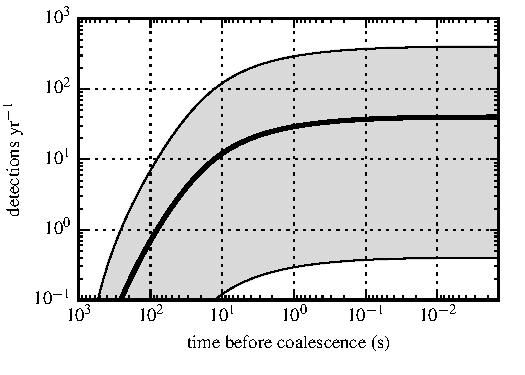
\includegraphics{figures/snr_in_time.pdf}
\caption{\label{fig:earlywarning} Expected number of NS--NS sources that will
be detectable $t$ seconds before coalescence.  The heavy solid line is the most
likely yearly rate estimate $\dot N_{\mathrm{re}}$ during Advanced \LIGO.  The
light solid lines represent the confidence interval $[\dot N_{\mathrm{low}}, \dot 
N_{\mathrm{high}}]$ described in
\cite{Abadie:2010p10836}.  Advanced \LIGO\ noise projections are described in 
\cite{ALIGONoise}.  Assuming that an \SNR\ of 8 is sufficient for
detection and that we observe $\dot N_{\mathrm{re}} = 40$ events~yr$^{-1}$ with a
detector in the `zero detuning, high power' configuration, about 10~yr$^{-1}$ will be 
detectable within 10 seconds before merger and $\sim1$~yr$^{-1}$ will be detectable 
within 100 seconds of merger.  The `zero detuning, lower power' and `\textsc{bbh} optimized' configurations are still more conducive to advance detection
but at the cost of fewer total detectable events above an \SNR\ of 8.}
\end{center}
\end{figure}

\editorial{Citation needed for LOOC-UP} The gravitational-wave community
initiated a project to send alerts when potential gravitational-wave transients
are observed.  In October 2010, \LIGO{} completed its sixth science run
(S6) and Virgo completed its third science run (VSR3).  While both
\textsc{ligo} detectors and Virgo were operating, several all-sky detection
pipelines operated in a low-latency configuration, namely \textsc{mbta}, ihope,
Coherent WaveBurst, and Omega~\cite{HugheyGWPAW2011, S6lowlatency}.
\editorial{Get references for these low-latency pipelines.} The S6 analyses
achieved latencies of 30--60 minutes, which were dominated by a human vetting
process. Candidates were sent for electromagnetic followup to several
telescopes; Swift, \textsc{rotse}, \textsc{tarot}, and Zadko~\cite{kanner2008,
HugheyGWPAW2011} took images of likely sky locations.  \textsc{mbta} achieved
the best gravitational-wave trigger generation latencies of 2--5 minutes.  We
assume that in the advanced detector era the vetting process will be automated,
so current gravitational wave search methodology and telescope actuation would
dominate latency.

Advance detection of compact binary coalescences (\CBC{}s) will require striking a balance between latency
and throughput.  \CBC{} searches consist of banks of matched filters, or
cross-correlations between the data stream and a bank of nominal ``template''
signals.  There are many different implementations of matched filters, but most
have high throughput at the cost of high latency, or low latency at the cost of
low throughput.  The former are epitomized by the overlap-save algorithm for
\textsc{fft} convolution, currently the preferred method in gravitational wave
searches.  The most obvious example of the latter is the time domain
(\textsc{td}) convolution, which has no latency at all.  However, its
computational complexity is quadratic in the length of the templates, so it is
prohibitively expensive for long templates.

Fortunately, the morphology of inspiral signals can be exploited to offset some
of the computational complexity of low latency algorithms.  First, the signals
evolve slowly in frequency, so that they can be broken into contiguous
band-limited time intervals and processed at possibly lower sample rates.
Second, inspiral filter banks consist of highly similar templates, admitting
principal component analysis to reduce the number of templates.  We described a
rank-reduction scheme based on singular value decomposition in
\cite{Cannon:2010p10398}.  We will use both aspects to demonstrate that a very
low latency analysis with advance detection of compact binary sources is
possible with current computing resources.  Assuming other technical sources of
latency can be reduced significantly, this should allow the possibility for
prompt alerts to be sent to the astronomical community.

The paper is organized as follows. First we provide an overview of our method
for detecting compact binary coalescence signals in an \earlywarning\ analysis.
We then describe the pipeline we have constructed that implements our method.
To validate the approach we present results of simulations and conclude with
some remarks on what remains to prepare for the Advanced detector era.

